%%%%%%%%%%%%%%%%%%%%%%%%%%%%%%%%%%%%%%%%%%%%%%%%%%%%%%%%%%%%%%%%%%%%%%
% Lớp 9 | Chương IV. Hệ thức lượng trong tam giác vuông | Một số hệ thức giữa cạnh, góc trong tam giác vuông và ứng dụng
% Dạng 9H4?12-3: Ứng dụng thực tế (đo chiều cao, khoảng cách)
%%%%%%%%%%%%%%%%%%%%%%%%%%%%%%%%%%%%%%%%%%%%%%%%%%%%%%%%%%%%%%%%%%%%%%


% nguồn: 2026-11-16_14_cum10_de1_cum10_de2_28_29 (nhập 16/11/2026)
\begin{bt}%[9H4V12-3]%[ma:0ff202f0]
% nguon: Cụm 10 – Đề tham khảo Tuyển sinh 10 năm học 2026-2027 TP.HCM – Đề số 29
Hai bạn Lâm và Dương rủ nhau đi câu cá bằng xe đạp từ nhà Lâm tại vị trí $A$ đến một hồ cá tại vị trí $B$. Trên đường đi, hai bạn phải vượt qua một con dốc có đỉnh ở vị trí $C$, chân đường vuông góc kẻ từ đỉnh dốc xuống mặt đất là $H$. Biết góc lên dốc là $\widehat{CAH} = 5^\circ$, góc xuống dốc là $\widehat{CBH} = 9^\circ$ và độ cao của con dốc là $CH = x\text{ (m)}$.
\begin{enumerate}[a)]
    \item Biểu diễn tổng quãng đường $S$ mà hai bạn đi từ $A$ đến $B$ theo $x$.
    \item Bạn Lâm đạp xe lên dốc với vận tốc $10\text{ km/h}$, mất $10$ phút thì đến đỉnh dốc, rồi từ đó thả dốc xuống với vận tốc $18\text{ km/h}$. Tính tổng thời gian hai bạn đi từ nhà đến hồ cá.
\end{enumerate}
\loigiai{
\begin{center}
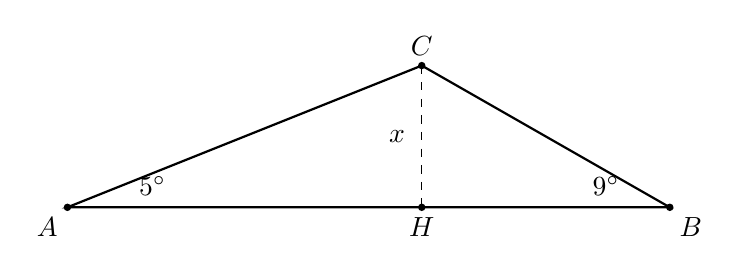
\begin{tikzpicture}[scale=0.9]
    \coordinate (H) at (0,0);
    \coordinate (C) at (0,2);
    \coordinate (A) at (-5,0);
    \coordinate (B) at (3.5,0);
    \draw[thick] (A) -- (C) -- (B) -- cycle;
    \draw[dashed] (C) -- (H);
    \node[below left] at (A) {$A$};
    \node[below right] at (B) {$B$};
    \node[above] at (C) {$C$};
    \node[below] at (H) {$H$};
    \node[left] at (-0.1,1) {$x$};
    \node at (-3.8,0.3) {$5^\circ$};
    \node at (2.6,0.3) {$9^\circ$};
    \fill (A) circle (1.5pt) (B) circle (1.5pt) (C) circle (1.5pt) (H) circle (1.5pt);
\end{tikzpicture}
\end{center}
\begin{enumerate}[a)]
    \item Trong tam giác vuông $AHC$ tại $H$:
    $$\sin A = \dfrac{CH}{AC} \implies AC = \dfrac{x}{\sin 5^\circ}\text{ (m)}.$$
    Trong tam giác vuông $BHC$ tại $H$:
    $$\sin B = \dfrac{CH}{BC} \implies BC = \dfrac{x}{\sin 9^\circ}\text{ (m)}.$$
    Tổng quãng đường $S$ hai bạn đi từ $A$ đến $B$ là:
    $$S = AC + BC = \dfrac{x}{\sin 5^\circ} + \dfrac{x}{\sin 9^\circ}\text{ (m)}.$$
    \item Đổi: $10\text{ phút} = \dfrac{1}{6}\text{ giờ}$.\\
    Chiều dài đoạn đường lên dốc $AC$ là:
    $$AC = v_1 \cdot t_1 = 10 \cdot \dfrac{1}{6} = \dfrac{5}{3}\text{ (km)}.$$
    Độ cao của con dốc là:
    $$CH = AC \cdot \sin 5^\circ = \dfrac{5}{3}\sin 5^\circ\text{ (km)}.$$
    Chiều dài đoạn đường xuống dốc $BC$ là:
    $$BC = \dfrac{CH}{\sin 9^\circ} = \dfrac{5\sin 5^\circ}{3\sin 9^\circ}\text{ (km)}.$$
    Thời gian hai bạn xuống dốc là:
    $$t_2 = \dfrac{BC}{v_2} = \dfrac{\dfrac{5\sin 5^\circ}{3\sin 9^\circ}}{18} = \dfrac{5\sin 5^\circ}{54\sin 9^\circ}\text{ (giờ)}.$$
    Tổng thời gian đi từ nhà đến hồ cá là:
    $$t = t_1 + t_2 = \dfrac{1}{6} + \dfrac{5\sin 5^\circ}{54\sin 9^\circ}\text{ (giờ)}.$$
    Đổi ra phút:
    $$t = \left(\dfrac{1}{6} + \dfrac{5\sin 5^\circ}{54\sin 9^\circ}\right) \cdot 60 = 10 + \dfrac{50\sin 5^\circ}{9\sin 9^\circ}\text{ (phút)} \approx 13{,}1\text{ phút (khoảng 13 phút 6 giây)}.$$
\end{enumerate}
}
\end{bt}

% nguồn: 2026-11-16_24_cum16_de2_cum16_de3_47_48 (nhập 16/11/2026)
\begin{bt}%[9H4V12-3]%[ma:44c1db4e]
% nguon: Đề tham khảo Tuyển sinh 10 năm học 2026-2027 Sở GD&ĐT TP.HCM - Cụm 16 - Đề 3 - Bài 4
Hôm chủ nhật vừa rồi, hai bạn Lâm và Dương rủ nhau đi câu cá. Lâm chở Dương bằng xe đạp từ nhà Lâm tại vị trí $A$ đến một hồ cá tại vị trí $B$. Trên đường đi phải băng qua một con dốc có đỉnh dốc ở vị trí $C$. Biết góc lên dốc $\widehat{CAH} = 5^\circ$, góc xuống dốc $\widehat{CBH} = 9^\circ$ và độ cao con dốc $CH = x\text{ (m)}$ ($H$ là hình chiếu của $C$ lên đường ngang $AB$).
\begin{enumerate}[a)]
	\item Biểu diễn theo $x$ quãng đường $S$ mà hai bạn đi từ nhà Lâm đến hồ cá.
	\item Bạn Lâm đạp xe lên dốc với vận tốc $10\text{ km/h}$, đi $10\text{ phút}$ thì đến đỉnh dốc, và từ đó thả dốc với vận tốc $18\text{ km/h}$. Tính thời gian hai bạn đi từ nhà đến điểm câu cá (theo phút và giây).
\end{enumerate}
\loigiai{
\begin{center}
	\begin{tikzpicture}[>=stealth, scale=1.2]
		\coordinate (A) at (0,0);
		\coordinate (H) at (4,0);
		\coordinate (B) at (6,0);
		\coordinate (C) at (4,1.5);
		\draw[thick] (A) -- (C) node[midway, above left] {lên dốc} -- (B) node[midway, above right] {xuống dốc};
		\draw[dashed] (A) -- (H) -- (B);
		\draw[dashed] (C) -- (H) node[midway, right] {$x\text{ (m)}$};
		\draw (3.7,0) -- (3.7,0.3) -- (4,0.3);
		\draw (0.8,0) arc (0:20:0.8) node[midway, right] {$5^\circ$};
		\draw (5.3,0) arc (180:143:0.7) node[midway, left] {$9^\circ$};
		\fill (A) circle (1.5pt) node[below] {$A$};
		\fill (B) circle (1.5pt) node[below] {$B$};
		\fill (C) circle (1.5pt) node[above] {$C$};
		\fill (H) circle (1.5pt) node[below] {$H$};
	\end{tikzpicture}
\end{center}
\begin{enumerate}[a)]
	\item Trong tam giác vuông $AHC$ vuông tại $H$, ta có:
	$$\sin A = \dfrac{CH}{AC} \implies AC = \dfrac{CH}{\sin 5^\circ} = \dfrac{x}{\sin 5^\circ}\text{ (m)}.$$
	Trong tam giác vuông $BHC$ vuông tại $H$, ta có:
	$$\sin B = \dfrac{CH}{BC} \implies BC = \dfrac{CH}{\sin 9^\circ} = \dfrac{x}{\sin 9^\circ}\text{ (m)}.$$
	Quãng đường $S$ mà hai bạn đi từ nhà đến hồ cá là:
	$$S = AC + BC = \dfrac{x}{\sin 5^\circ} + \dfrac{x}{\sin 9^\circ}\text{ (m)}.$$
	\item Đổi $10\text{ phút} = \dfrac{10}{60}\text{ giờ} = \dfrac{1}{6}\text{ giờ}$.\\
	Quãng đường Lâm đạp xe lên dốc (đoạn $AC$) là:
	$$AC = v_1 \cdot t_1 = 10 \cdot \dfrac{1}{6} = \dfrac{5}{3}\text{ (km)}.$$
	Độ cao con dốc là:
	$$CH = AC \cdot \sin 5^\circ = \dfrac{5}{3} \cdot \sin 5^\circ\text{ (km)}.$$
	Quãng đường thả dốc (đoạn $BC$) là:
	$$BC = \dfrac{CH}{\sin 9^\circ} = \dfrac{5\sin 5^\circ}{3\sin 9^\circ}\text{ (km)}.$$
	Thời gian thả dốc (đoạn $BC$) là:
	$$t_2 = \dfrac{BC}{v_2} = \dfrac{5\sin 5^\circ}{3\sin 9^\circ} : 18 = \dfrac{5\sin 5^\circ}{54\sin 9^\circ}\text{ (giờ)}.$$
	Đổi ra phút:
	$$t_2 = \dfrac{5\sin 5^\circ}{54\sin 9^\circ} \cdot 60 = \dfrac{50\sin 5^\circ}{9\sin 9^\circ} \approx 3{,}1\text{ (phút)} \approx 3\text{ phút } 6\text{ giây}.$$
	Tổng thời gian hai bạn đi từ nhà đến hồ cá là:
	$$t = t_1 + t_2 = 10\text{ phút} + 3\text{ phút } 6\text{ giây} = 13\text{ phút } 6\text{ giây}.$$
\end{enumerate}
}
\end{bt}
